% Options for packages loaded elsewhere
\PassOptionsToPackage{unicode}{hyperref}
\PassOptionsToPackage{hyphens}{url}
%
\documentclass[
  11pt,
]{article}
\usepackage{amsmath,amssymb}
\usepackage{iftex}
\ifPDFTeX
  \usepackage[T1]{fontenc}
  \usepackage[utf8]{inputenc}
  \usepackage{textcomp} % provide euro and other symbols
\else % if luatex or xetex
  \usepackage{unicode-math} % this also loads fontspec
  \defaultfontfeatures{Scale=MatchLowercase}
  \defaultfontfeatures[\rmfamily]{Ligatures=TeX,Scale=1}
\fi
\usepackage{lmodern}
\ifPDFTeX\else
  % xetex/luatex font selection
  \setmainfont[]{Latin Modern Roman}
\fi
% Use upquote if available, for straight quotes in verbatim environments
\IfFileExists{upquote.sty}{\usepackage{upquote}}{}
\IfFileExists{microtype.sty}{% use microtype if available
  \usepackage[]{microtype}
  \UseMicrotypeSet[protrusion]{basicmath} % disable protrusion for tt fonts
}{}
\makeatletter
\@ifundefined{KOMAClassName}{% if non-KOMA class
  \IfFileExists{parskip.sty}{%
    \usepackage{parskip}
  }{% else
    \setlength{\parindent}{0pt}
    \setlength{\parskip}{6pt plus 2pt minus 1pt}}
}{% if KOMA class
  \KOMAoptions{parskip=half}}
\makeatother
\usepackage{xcolor}
\usepackage[margin=2.5cm]{geometry}
\usepackage{listings}
\newcommand{\passthrough}[1]{#1}
\lstset{defaultdialect=[5.3]Lua}
\lstset{defaultdialect=[x86masm]Assembler}
\usepackage{longtable,booktabs,array}
\usepackage{calc} % for calculating minipage widths
% Correct order of tables after \paragraph or \subparagraph
\usepackage{etoolbox}
\makeatletter
\patchcmd\longtable{\par}{\if@noskipsec\mbox{}\fi\par}{}{}
\makeatother
% Allow footnotes in longtable head/foot
\IfFileExists{footnotehyper.sty}{\usepackage{footnotehyper}}{\usepackage{footnote}}
\makesavenoteenv{longtable}
\usepackage{graphicx}
\makeatletter
\def\maxwidth{\ifdim\Gin@nat@width>\linewidth\linewidth\else\Gin@nat@width\fi}
\def\maxheight{\ifdim\Gin@nat@height>\textheight\textheight\else\Gin@nat@height\fi}
\makeatother
% Scale images if necessary, so that they will not overflow the page
% margins by default, and it is still possible to overwrite the defaults
% using explicit options in \includegraphics[width, height, ...]{}
\setkeys{Gin}{width=\maxwidth,height=\maxheight,keepaspectratio}
% Set default figure placement to htbp
\makeatletter
\def\fps@figure{htbp}
\makeatother
\setlength{\emergencystretch}{3em} % prevent overfull lines
\providecommand{\tightlist}{%
  \setlength{\itemsep}{0pt}\setlength{\parskip}{0pt}}
\setcounter{secnumdepth}{-\maxdimen} % remove section numbering
\ifLuaTeX
\usepackage[bidi=basic]{babel}
\else
\usepackage[bidi=default]{babel}
\fi
\babelprovide[main,import]{spanish}
\ifPDFTeX
\else
\babelfont{rm}[]{Latin Modern Roman}
\fi
% get rid of language-specific shorthands (see #6817):
\let\LanguageShortHands\languageshorthands
\def\languageshorthands#1{}
\usepackage{float}
\usepackage{needspace}
\usepackage{fvextra}
\usepackage{listings}
\lstset{basicstyle=\ttfamily\footnotesize,breaklines=true,columns=fullflexible,keepspaces=true,showstringspaces=false,frame=none}
\floatplacement{figure}{H}
\pagestyle{plain}
\setlength{\parindent}{0pt}
\setlength{\parskip}{6pt}
\renewcommand{\arraystretch}{1.15}
\AtBeginEnvironment{longtable}{\footnotesize}
\ifLuaTeX
  \usepackage{selnolig}  % disable illegal ligatures
\fi
\IfFileExists{bookmark.sty}{\usepackage{bookmark}}{\usepackage{hyperref}}
\IfFileExists{xurl.sty}{\usepackage{xurl}}{} % add URL line breaks if available
\urlstyle{same}
\hypersetup{
  pdflang={es},
  hidelinks,
  pdfcreator={LaTeX via pandoc}}

\author{}
\date{}

\begin{document}

\begin{titlepage}
\centering
{\large Universidad de Concepción\par}
\vspace{0.3cm}
Facultad de Ingeniería\\
Departamento de Informática y Ciencias de la Computación
\vspace{2.8cm}

{\LARGE\bfseries Laboratorio Evaluado N.º 3\par}
\vspace{0.8cm}
{\Large Validación, almacenamiento y análisis de integridad de telemetría en un nodo CPS\par}
\vspace{2.4cm}

{\large\bfseries Integrantes\par}
\vspace{0.4cm}
Agustín Salgado Espinoza\\[0.2cm]
Sebastián Garcias Cabrera
\vfill
Análisis y Diseño de Sistemas Ciber-Físicos\\
Semestre 2026-2\\[0.5cm]
16 de octubre de 2026
\end{titlepage}
\setcounter{page}{1}

\hypertarget{validaciuxf3n-de-tramas}{%
\section{1. Validación de tramas}\label{validaciuxf3n-de-tramas}}

La función \passthrough{\lstinline!validar(linea)!}, implementada en
\passthrough{\lstinline!pipeline.py!}, devuelve los campos numéricos y
\passthrough{\lstinline!ok!} cuando la trama supera las verificaciones;
en caso contrario, retorna \passthrough{\lstinline!None!} y la primera
causa de rechazo según esta prioridad:

\begin{enumerate}
\def\labelenumi{\arabic{enumi}.}
\tightlist
\item
  \textbf{basura:} el texto recibido no comienza con
  \passthrough{\lstinline!$!}.
\item
  \textbf{truncada:} no existe \passthrough{\lstinline!*!} o el checksum
  no consta exactamente de dos caracteres hexadecimales.
\item
  \textbf{checksum:} el XOR de los códigos de los caracteres entre
  \passthrough{\lstinline!$!} y \passthrough{\lstinline!*!}, sin incluir
  estos delimitadores, difiere del checksum recibido.
\item
  \textbf{formato:} el identificador no es
  \passthrough{\lstinline!CPS!}, el cuerpo no contiene siete campos o no
  se pueden convertir los campos a sus tipos numéricos correspondientes.
\end{enumerate}

\passthrough{\lstinline!seq!}, \passthrough{\lstinline!t\_ms!},
\passthrough{\lstinline!a0!}, \passthrough{\lstinline!pulsos!} y
\passthrough{\lstinline!boton!} se convierten a enteros;
\passthrough{\lstinline!t\_mcu!}, a real finito. Esta función no evalúa
continuidad temporal ni plausibilidad física. Por lo tanto, una medición
alterada con checksum recalculado puede ser aceptada.

El archivo tiene 868 líneas en total, de las cuales dos son comentarios.

\Needspace{4.5cm}
\begin{longtable}[]{@{}lr@{}}
\toprule\noalign{}
Clasificación & Cantidad \\
\midrule\noalign{}
\endhead
\bottomrule\noalign{}
\endlastfoot
Líneas de datos, excluidos comentarios & 866 \\
Tramas válidas & 850 \\
Rechazos por basura & 3 \\
Rechazos por truncada & 4 \\
Rechazos por checksum & 9 \\
Rechazos por formato & 0 \\
Rechazos totales & 16 \\
\end{longtable}

Se comprueba que 850 + 3 + 4 + 9 + 0 = 866. La ausencia de rechazos por
\passthrough{\lstinline!formato!} en la captura no elimina la necesidad
de implementar esa condición.

\textbf{Codificación.} El archivo debe abrirse con
\passthrough{\lstinline!encoding="utf-8"!} porque ese es su formato
declarado y contiene caracteres no ASCII en las líneas de basura.
Depender de la codificación predeterminada del sistema puede producir
una decodificación incorrecta o una excepción, según el entorno.
Especificar UTF-8 permite conservar fielmente el texto recibido para su
almacenamiento y análisis. No se usa
\passthrough{\lstinline!errors="ignore"!} ni una sustitución adicional
de caracteres.

\hypertarget{almacenamiento-en-sqlite}{%
\section{2. Almacenamiento en SQLite}\label{almacenamiento-en-sqlite}}

Se generó \passthrough{\lstinline!cps\_lab3.db!} con el esquema exacto
del enunciado. Las 850 tramas válidas se insertaron en
\passthrough{\lstinline!tramas!} y las 16 líneas rechazadas, en
\passthrough{\lstinline!rechazos!}, conservando el orden de aparición
dentro de cada tabla. Los \passthrough{\lstinline!id!} son correlativos
e independientes en ambas tablas, como en el respaldo.
\passthrough{\lstinline!ts!} conserva el texto de la marca temporal y
\passthrough{\lstinline!linea!} conserva el texto recibido, sin la hora
y sin el terminador de línea.

Las dos cargas se realizaron con \passthrough{\lstinline!executemany!},
dentro de una única transacción explícita con
\passthrough{\lstinline!BEGIN!}, \passthrough{\lstinline!commit()!} al
terminar y \passthrough{\lstinline!rollback()!} ante un error.

\begin{lstlisting}[language=SQL]
SELECT COUNT(*) AS n_tramas FROM tramas;      -- 850
SELECT COUNT(*) AS n_rechazos FROM rechazos;  -- 16
SELECT causa, COUNT(*) AS cantidad FROM rechazos GROUP BY causa;
\end{lstlisting}

Una transacción única evita confirmar cada fila por separado, lo que
reduce la sobrecarga de sincronización y escritura. Además, asegura
atomicidad: se confirma la carga completa o se revierte, evitando una
base parcialmente cargada.

Los rechazos se almacenan porque son evidencia de la calidad del canal y
de incidentes de operación. Permiten calcular la cantidad de tramas
dañadas, correlacionar el ruido con las reconexiones y revisar las
decisiones del validador. Descartarlos impediría distinguir corrupción
de pérdidas y reduciría la trazabilidad.

\hypertarget{verificaciuxf3n-cruzada}{%
\section{3. Verificación cruzada}\label{verificaciuxf3n-cruzada}}

Se adjuntó la base de respaldo mediante
\passthrough{\lstinline!ATTACH DATABASE!} y se compararon ambas bases
mediante las consultas incluidas en
\passthrough{\lstinline!consultas.sql!}.

\Needspace{4.5cm}
\begin{longtable}[]{@{}lrr@{}}
\toprule\noalign{}
Indicador & Base generada & Respaldo \\
\midrule\noalign{}
\endhead
\bottomrule\noalign{}
\endlastfoot
Cantidad de tramas & 850 & 850 \\
Suma de seq & 99647 & 99647 \\
Suma de a0 & 482689 & 482689 \\
Rechazos por basura & 3 & 3 \\
Rechazos por truncada & 4 & 4 \\
Rechazos por checksum & 9 & 9 \\
Rechazos por formato & 0 & 0 \\
\end{longtable}

\begin{lstlisting}[language=SQL]
ATTACH DATABASE 'cps_lab3_respaldo.db' AS ref;

SELECT ts,seq,t_ms,t_mcu,a0,pulsos,boton FROM main.tramas
EXCEPT
SELECT ts,seq,t_ms,t_mcu,a0,pulsos,boton FROM ref.tramas;

SELECT ts,seq,t_ms,t_mcu,a0,pulsos,boton FROM ref.tramas
EXCEPT
SELECT ts,seq,t_ms,t_mcu,a0,pulsos,boton FROM main.tramas;
\end{lstlisting}

Ambas consultas retornan \textbf{cero filas}. Se verificaron también los
rechazos en ambos sentidos y la igualdad completa de ambas tablas
ordenadas por \passthrough{\lstinline!id!}. Esta última comprobación
incluye orden y multiplicidad, que \passthrough{\lstinline!EXCEPT!} por
sí solo no comprueba. No se encontraron diferencias que requirieran
corregir el validador.

\hypertarget{disponibilidad-por-tramas}{%
\section{4. Disponibilidad por tramas}\label{disponibilidad-por-tramas}}

Se numeraron las sesiones con una suma acumulada que aumenta cuando
\passthrough{\lstinline!seq = 1!}, siguiendo el criterio del enunciado:

\begin{lstlisting}[language=SQL]
WITH numeradas AS (
  SELECT *, SUM(CASE WHEN seq = 1 THEN 1 ELSE 0 END)
    OVER (ORDER BY id ROWS BETWEEN UNBOUNDED PRECEDING AND CURRENT ROW) AS sesion
  FROM tramas
)
SELECT sesion, COUNT(*) AS n_validas, MAX(seq) AS max_seq,
       MIN(ts) AS primera_ts, MAX(ts) AS ultima_ts
FROM numeradas
GROUP BY sesion ORDER BY sesion;
\end{lstlisting}

No se considera cada descenso de \passthrough{\lstinline!seq!} como un
reinicio: existen descensos que requieren el análisis de seguridad de la
pregunta 9. En esta pregunta se mantienen todas las tramas
sintácticamente válidas, tal como exige el enunciado.

\Needspace{4.5cm}
\begin{longtable}[]{@{}
  >{\raggedright\arraybackslash}p{(\columnwidth - 8\tabcolsep) * \real{0.1765}}
  >{\raggedright\arraybackslash}p{(\columnwidth - 8\tabcolsep) * \real{0.1765}}
  >{\raggedright\arraybackslash}p{(\columnwidth - 8\tabcolsep) * \real{0.1765}}
  >{\raggedleft\arraybackslash}p{(\columnwidth - 8\tabcolsep) * \real{0.2353}}
  >{\raggedleft\arraybackslash}p{(\columnwidth - 8\tabcolsep) * \real{0.2353}}@{}}
\toprule\noalign{}
\begin{minipage}[b]{\linewidth}\raggedright
Sesión
\end{minipage} & \begin{minipage}[b]{\linewidth}\raggedright
Primera trama válida (hora)
\end{minipage} & \begin{minipage}[b]{\linewidth}\raggedright
Última trama válida (hora)
\end{minipage} & \begin{minipage}[b]{\linewidth}\raggedleft
Nval
\end{minipage} & \begin{minipage}[b]{\linewidth}\raggedleft
Máximo seq
\end{minipage} \\
\midrule\noalign{}
\endhead
\bottomrule\noalign{}
\endlastfoot
1 & 15:00:01.604 & 15:10:59.723 & 319 & 330 \\
2 & 15:11:18.725 & 15:17:30.793 & 182 & 187 \\
3 & 15:17:55.623 & 15:24:59.700 & 211 & 213 \\
4 & 15:25:15.424 & 15:29:59.476 & 138 & 143 \\
\end{longtable}

Todas las horas corresponden al 8 de octubre de 2026.

\begin{itemize}
\tightlist
\item
  Nesp = 330 + 187 + 213 + 143 = \textbf{873}.
\item
  Nval = \textbf{850}.
\item
  Ncorr = 9 por checksum + 4 truncadas = \textbf{13}.
\item
  Nperd = 873 - 850 - 13 = \textbf{10}.
\item
  D = 100 × 850 / 873 = \textbf{97,3654 \%}.
\end{itemize}

\Needspace{4.5cm}
\begin{longtable}[]{@{}rrrrrr@{}}
\toprule\noalign{}
N.º de sesiones & Nesp & Nval & Ncorr & Nperd & D {[}\%{]} \\
\midrule\noalign{}
\endhead
\bottomrule\noalign{}
\endlastfoot
4 & 873 & 850 & 13 & 10 & 97,3654 \\
\end{longtable}

Las líneas de basura no se consideran tramas porque no comienzan con el
delimitador \passthrough{\lstinline!$!} y no aportan evidencia de una
muestra estructurada del Arduino. Un fragmento de ruido no debe contarse
como una trama emitida y dañada. En cambio, las categorías checksum y
truncada se contabilizan como tramas dañadas según la definición de
Ncorr del laboratorio.

\hypertarget{throughput-y-temporizaciuxf3n}{%
\section{5. Throughput y
temporización}\label{throughput-y-temporizaciuxf3n}}

\hypertarget{a.-throughput-largo-medio-y-ocupaciuxf3n}{%
\subsection{5a. Throughput, largo medio y
ocupación}\label{a.-throughput-largo-medio-y-ocupaciuxf3n}}

Se utilizaron las marcas temporales de la primera y última trama válida:

\begin{itemize}
\tightlist
\item
  Primera: \textbf{2026-10-08 15:00:01.604}.
\item
  Última: \textbf{2026-10-08 15:29:59.476}.
\item
  T = \textbf{1797,872 s}.
\end{itemize}

El largo de cada trama se midió directamente sobre el texto válido del
archivo crudo, desde \passthrough{\lstinline!$!} hasta el último dígito
del checksum, y se sumaron dos bytes por
\passthrough{\lstinline!\\r\\n!}. No se reconstruyeron las tramas desde
SQLite para evitar alterar su representación numérica original. Las
tramas válidas son ASCII, por lo que su codificación UTF-8 utiliza un
byte por carácter.

La suma de los largos de las 850 tramas válidas, incluido CRLF, es
\textbf{27732 bytes}. Los largos individuales van de 29 a 35 bytes.

\Needspace{4.5cm}
\begin{longtable}[]{@{}llr@{}}
\toprule\noalign{}
Magnitud & Cálculo & Resultado \\
\midrule\noalign{}
\endhead
\bottomrule\noalign{}
\endlastfoot
X & 850 / 1797,872 & 0,472781 tramas/s \\
L & 27732 / 850 & 32,625882 bytes/trama \\
R & 10 × L × X & 154,249023 bit/s \\
\ensuremath{\rho} & 100 × R / 115200 & 0,133897 \% \\
\end{longtable}

La ocupación calculada es muy baja: el margen nominal restante es
aproximadamente \textbf{99,8661 \%}, por lo que existe margen de ancho
de banda para agregar campos de nuevos sensores. Este cálculo representa
el tráfico válido según la fórmula solicitada; no incluye el tráfico
rechazado ni garantiza capacidad de muestreo, procesamiento o fiabilidad
del nodo. Agregar sensores requiere comprobar también esas
restricciones.

\hypertarget{b.-distribuciuxf3n-de-los-intervalos}{%
\subsection{5b. Distribución de los
intervalos}\label{b.-distribuciuxf3n-de-los-intervalos}}

Se calculó Δt entre marcas \passthrough{\lstinline!ts!} consecutivas, en
orden de \passthrough{\lstinline!id!}. Las 850 tramas generan
\textbf{849 intervalos}, sin eliminar las separaciones entre sesiones.

\begin{figure}
\centering
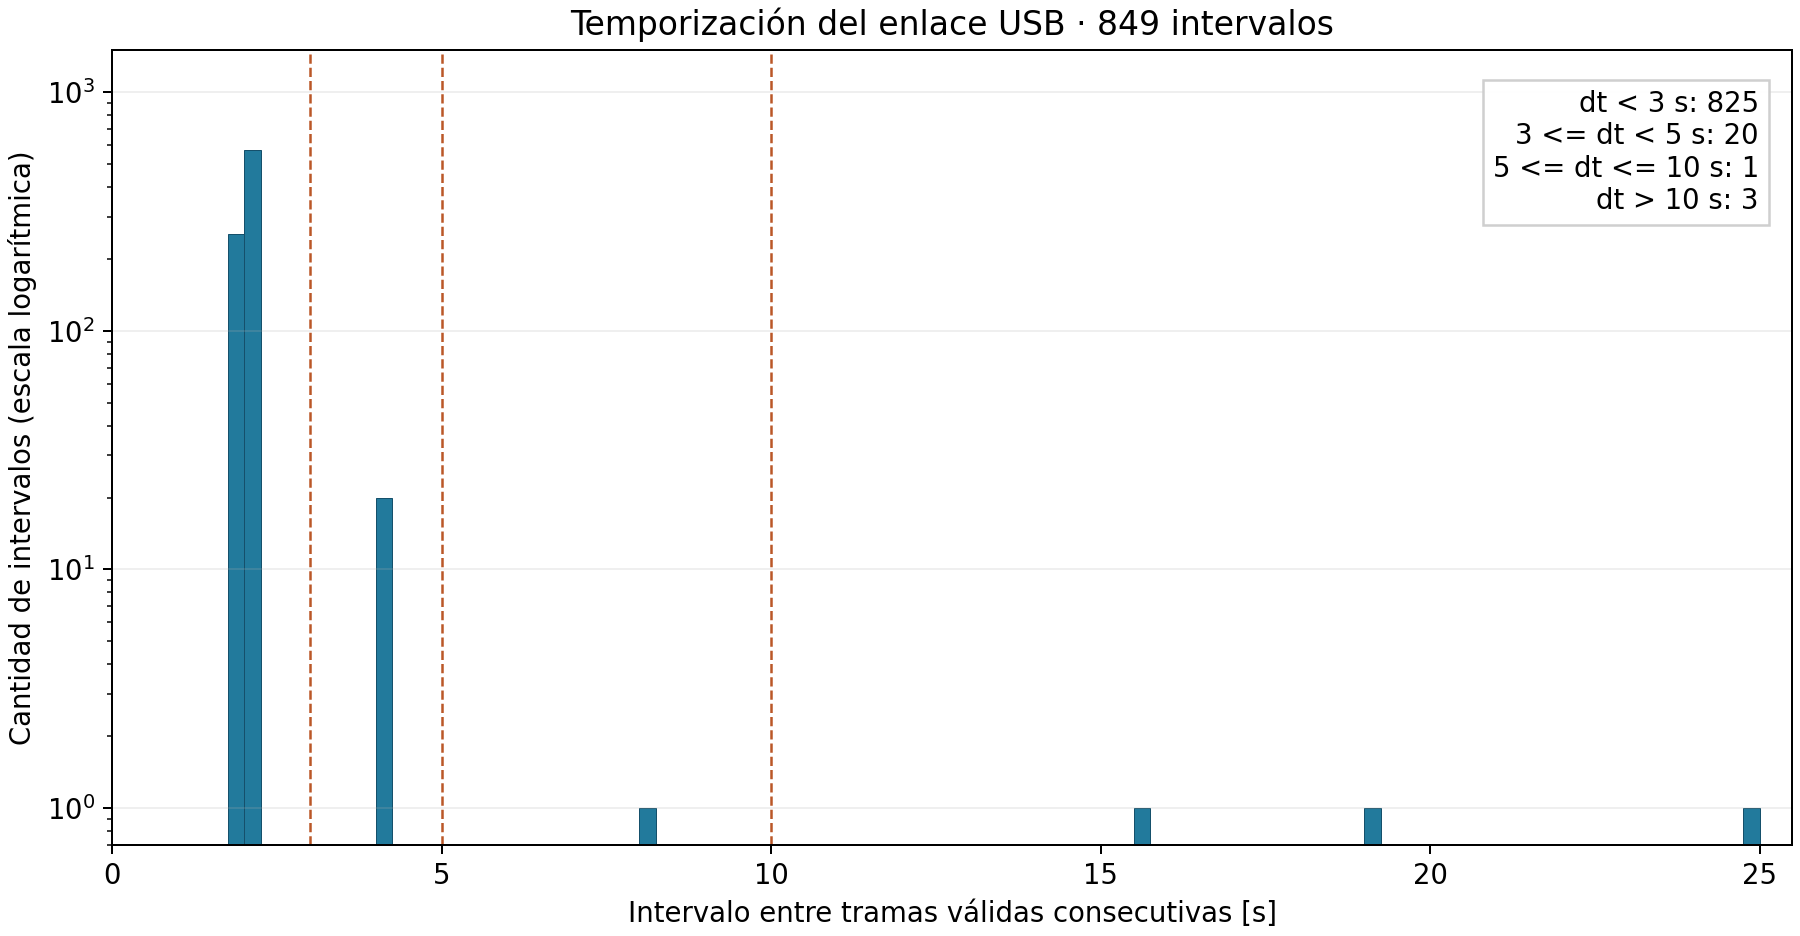
\includegraphics{figuras/histograma_intervalos.png}
\caption{Histograma de los intervalos entre tramas válidas, con eje
vertical logarítmico}
\end{figure}

\Needspace{7cm}
\begin{longtable}[]{@{}
  >{\raggedright\arraybackslash}p{(\columnwidth - 4\tabcolsep) * \real{0.2200}}
  >{\raggedleft\arraybackslash}p{(\columnwidth - 4\tabcolsep) * \real{0.1200}}
  >{\raggedright\arraybackslash}p{(\columnwidth - 4\tabcolsep) * \real{0.6600}}@{}}
\toprule\noalign{}
\begin{minipage}[b]{\linewidth}\raggedright
Categoría
\end{minipage} & \begin{minipage}[b]{\linewidth}\raggedleft
Cantidad
\end{minipage} & \begin{minipage}[b]{\linewidth}\raggedright
Interpretación respaldada por la captura
\end{minipage} \\
\midrule\noalign{}
\endhead
\bottomrule\noalign{}
\endlastfoot
Δt \textless{} 3 s & 825 & Recepción a la cadencia nominal de unos 2 s,
con pequeñas variaciones de temporización. La cadencia por sí sola no
garantiza legitimidad del contenido. \\
3 \ensuremath{\leq} Δt \textless{} 5 s & 20 & Intervalos cercanos a 4 s: falta una trama
válida intermedia. En 13 casos aparece un rechazo por checksum o
truncada entre las dos válidas; en los otros 7 no se recibió la trama
intermedia. \\
5 \ensuremath{\leq} Δt \ensuremath{\leq} 10 s & 1 & Intervalo de 8,001 s, entre seq 31 y 35 en la sesión
1: faltan tres tramas consecutivas (32, 33 y 34), sin rechazos
intermedios. \\
Δt \textgreater{} 10 s & 3 & Interrupciones de 19,002 s, 24,830 s y
15,724 s, acompañadas de reinicio de seq y t\_ms y de una línea de
basura antes de la primera trama de la nueva sesión. Son compatibles con
desconexiones y reaperturas USB; se desarrollan en P6. \\
\end{longtable}

La interpretación temporal concuerda con los conteos: 7 pérdidas
aisladas + 3 pérdidas consecutivas = 10 tramas nunca recibidas; los
otros 13 intervalos de aproximadamente 4 s corresponden a las 13 tramas
dañadas. El histograma usa intervalos de clase de 0,25 s y escala
logarítmica vertical para que se aprecien tanto la concentración cerca
de 2 s como los eventos poco frecuentes.

\hypertarget{desconexiones-y-disponibilidad-operacional}{%
\section{6. Desconexiones y disponibilidad
operacional}\label{desconexiones-y-disponibilidad-operacional}}

\hypertarget{a.-identificaciuxf3n-de-fallas}{%
\subsection{6a. Identificación de
fallas}\label{a.-identificaciuxf3n-de-fallas}}

Se identifican tres desconexiones. En cada una coinciden cuatro señales:
una separación de recepción superior a 10 s (frente a 2 s nominales),
seq reiniciada en 1, t\_ms reiniciado cerca de 2000 ms y una línea de
basura entre las dos tramas válidas. Los contadores acumulados se
reinician; boton vuelve de 31 a 0 en la primera reconexión. No se
clasifica como desconexión un simple retroceso de seq.

\Needspace{4.5cm}
\begin{longtable}[]{@{}
  >{\raggedright\arraybackslash}p{(\columnwidth - 6\tabcolsep) * \real{0.2308}}
  >{\raggedright\arraybackslash}p{(\columnwidth - 6\tabcolsep) * \real{0.2308}}
  >{\raggedright\arraybackslash}p{(\columnwidth - 6\tabcolsep) * \real{0.2308}}
  >{\raggedleft\arraybackslash}p{(\columnwidth - 6\tabcolsep) * \real{0.3077}}@{}}
\toprule\noalign{}
\begin{minipage}[b]{\linewidth}\raggedright
Falla
\end{minipage} & \begin{minipage}[b]{\linewidth}\raggedright
Última válida previa (08-10-2026)
\end{minipage} & \begin{minipage}[b]{\linewidth}\raggedright
Primera válida posterior (08-10-2026)
\end{minipage} & \begin{minipage}[b]{\linewidth}\raggedleft
Reparación {[}s{]}
\end{minipage} \\
\midrule\noalign{}
\endhead
\bottomrule\noalign{}
\endlastfoot
1 & 15:10:59.723 & 15:11:18.725 & 19,002 \\
2 & 15:17:30.793 & 15:17:55.623 & 24,830 \\
3 & 15:24:59.700 & 15:25:15.424 & 15,724 \\
\end{longtable}

Las líneas de basura aparecen a las 15:11:15.150, 15:17:52.050 y
15:25:11.850. La tabla usa la última trama antes de cada falla y la
primera después de la recuperación, como indica el enunciado. La captura
no permite saber el instante exacto en que se desconectó el cable.

\hypertarget{b.-indicadores-operacionales}{%
\subsection{6b. Indicadores
operacionales}\label{b.-indicadores-operacionales}}

Tiempo total de reparación = 59,556 s. Tiempo operativo = 1797,872 -
59,556 = 1738,316 s.

\begin{itemize}
\tightlist
\item
  MTTR = 59,556 / 3 = \textbf{19,852 s}.
\item
  MTBF = 1738,316 / 3 = \textbf{579,438667 s}.
\item
  A = 100 × 579,438667 / (579,438667 + 19,852) = \textbf{96,6874 \%}.
\end{itemize}

A es menor que D = 97,3654 \%. A mide la fracción temporal operativa
penalizando los intervalos de desconexión. D mide la fracción de tramas
estimadas como emitidas que se validaron: penaliza corrupción y
pérdidas, pero su denominador no representa las muestras que podrían
haberse producido durante una desconexión. Ninguna de las dos métricas
distingue por sí sola los ataques que mantienen un formato correcto.

\hypertarget{falla-de-sensor-entrada-a0-flotante}{%
\section{7. Falla de sensor: entrada A0
flotante}\label{falla-de-sensor-entrada-a0-flotante}}

\hypertarget{a.-gruxe1fico-y-regla-automuxe1tica}{%
\subsection{7a. Gráfico y regla
automática}\label{a.-gruxe1fico-y-regla-automuxe1tica}}

\begin{figure}
\centering
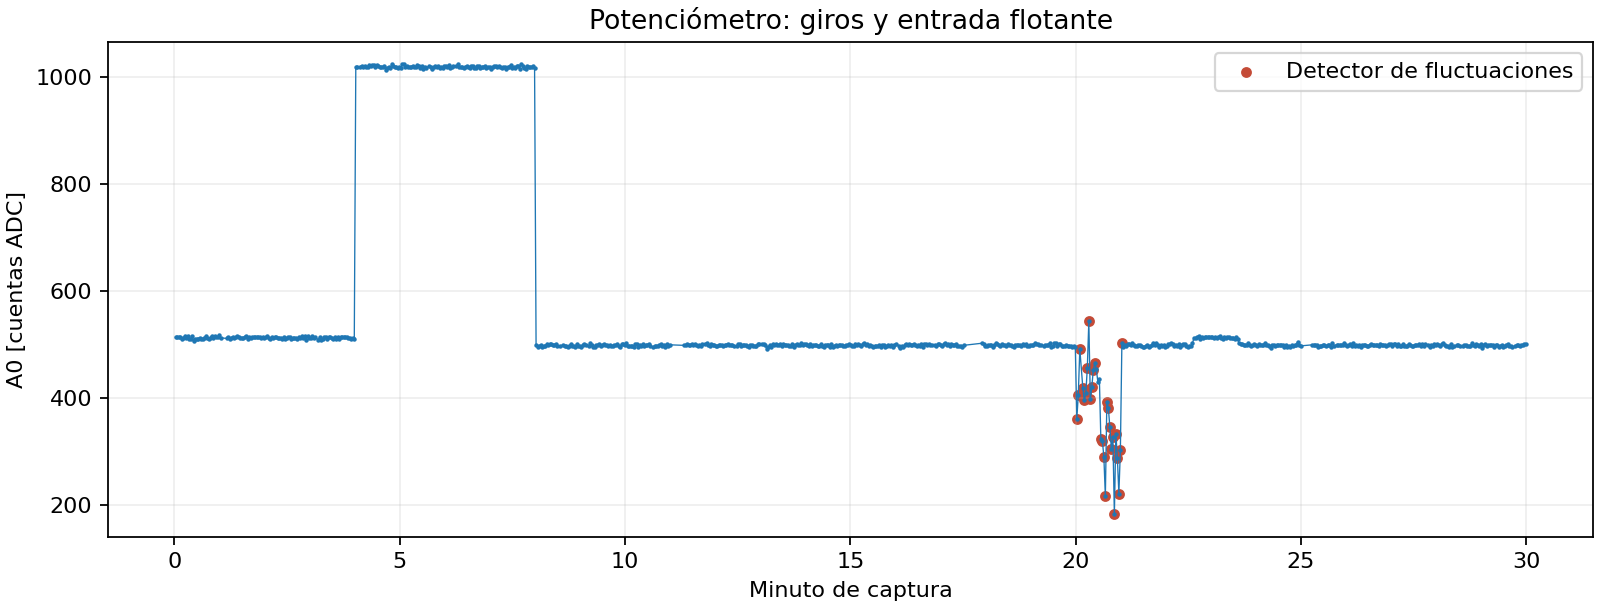
\includegraphics{figuras/sensor_a0.png}
\caption{Lectura de A0 y marcas del detector}
\end{figure}

Se define b{[}k{]} = 1 si \textbar a0{[}k{]} - a0{[}k-1{]}\textbar{}
\textgreater{} 20 cuentas, y 0 en otro caso. Se marca la trama k cuando
al menos 3 de las 5 diferencias b{[}k-2{]}, \ldots, b{[}k+2{]} superan
ese umbral. La ventana está centrada en la muestra evaluada, por lo que
necesita dos muestras posteriores. Por eso, esta regla sirve para
revisar la captura y tiene un retraso si se usa durante la recepción.
Una ventana debe estar completa para evaluarse.

Un giro intencional genera un salto aislado seguido de valores estables;
la entrada flotante genera saltos repetidos. La regla se aplica a toda
la captura, sin imponer de antemano la ventana de falla.

\Needspace{4.5cm}
\begin{longtable}[]{@{}ll@{}}
\toprule\noalign{}
Resultado & Valor \\
\midrule\noalign{}
\endhead
\bottomrule\noalign{}
\endlastfoot
Primera marca & 15:20:01.647; minuto 20,027450; seq 64 \\
Última marca & 15:21:01.658; minuto 21,027633; seq 94 \\
Total de tramas marcadas & 27 \\
Marcas fuera de ese intervalo & 0 \\
Falsos positivos en los giros de los minutos 4 y 8 & 0 \\
\end{longtable}

El intervalo comprendido entre la primera y la última marca es
20,027450-21,027633 min, pero no todas las muestras de ese intervalo
están marcadas: quedan sin marcar los ids 576, 577 y 578. Visualmente,
el tramo fluctuante termina en 15:20:59.656 (20,994267 min), y en
15:21:01.658 el sensor ya retorna a 502 cuentas. Por tanto, respecto de
ese tramo observado, hay \textbf{26 aciertos, 3 omisiones y 1 falso
positivo de borde}. No hay otras marcas fuera del tramo de falla. El
filtro incluye la primera muestra de recuperación debido al salto final;
esto explica el pequeño exceso del límite detectado. En el segmento
fluctuante se observan valores entre 182 y 543, frente al nivel cercano
a 498 anterior y posterior.

\hypertarget{b.-sintaxis-frente-a-fuxedsica}{%
\subsection{7b. Sintaxis frente a
física}\label{b.-sintaxis-frente-a-fuxedsica}}

validar() acepta esas tramas porque conservan delimitadores, campos
numéricos y checksum correcto. Incluso sus lecturas están dentro del
rango ADC 0-1023. La validación sintáctica comprueba que el mensaje
llegó con estructura e integridad accidental correctas; la física
examina si su contenido es coherente con el sensor y el proceso. Un dato
físicamente incorrecto puede viajar sin errores de comunicación.

\hypertarget{inyecciuxf3n-de-datos-falsos-fdi}{%
\section{8. Inyección de datos falsos
(FDI)}\label{inyecciuxf3n-de-datos-falsos-fdi}}

\hypertarget{a.-variable-luxedmites-y-magnitud}{%
\subsection{8a. Variable, límites y
magnitud}\label{a.-variable-luxedmites-y-magnitud}}

La variable afectada es t\_mcu. Se identifica un bloque de \textbf{48
tramas}, todas sintácticamente válidas, entre los siguientes extremos:

\Needspace{4.5cm}
\begin{longtable}[]{@{}llrr@{}}
\toprule\noalign{}
Extremo & ts (08-10-2026) & seq & Minuto \\
\midrule\noalign{}
\endhead
\bottomrule\noalign{}
\endlastfoot
Primera alterada & 15:14:12.754 & 88 & 14,212567 \\
Última alterada & 15:15:46.770 & 135 & 15,779500 \\
\end{longtable}

\begin{figure}
\centering
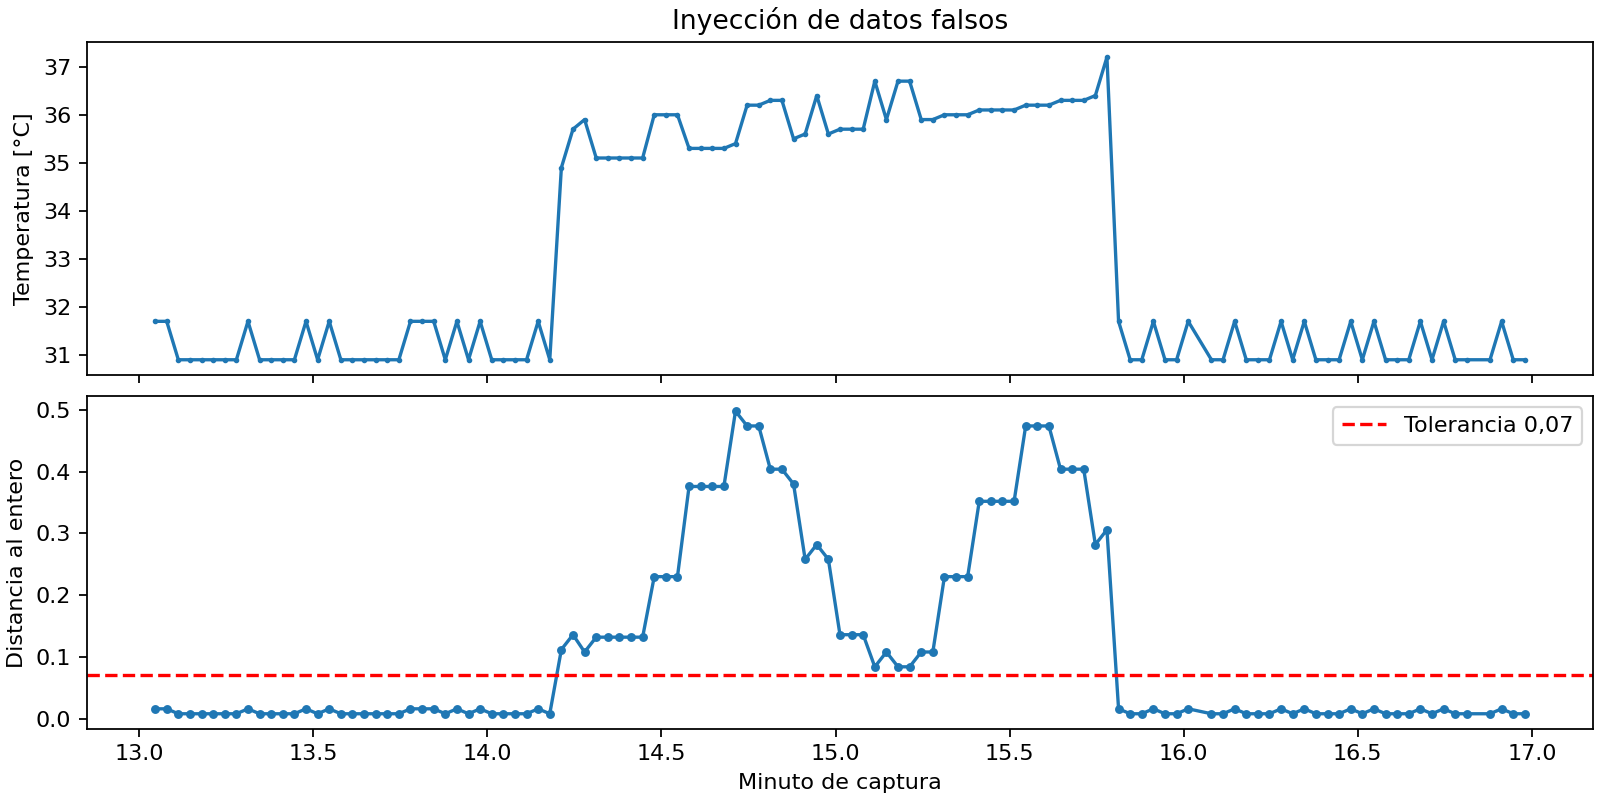
\includegraphics{figuras/fdi.png}
\caption{Temperatura alterada y prueba de cuantización ADC}
\end{figure}

Como referencia se usan las tramas de los minutos 13-14,2 y 15,8-17, sin
incluir el bloque alterado. Sus temperaturas medias son 31,151429 °C y
31,158824 °C. El promedio de ambos niveles es 31,155126 °C, mientras que
el bloque alterado promedia 35,897917 °C: \textbf{elevación media
estimada de 4,742791 °C}. El bloque va de 34,9 a 37,2 °C,
aproximadamente +3,745 a +6,045 °C respecto del nivel de referencia. La
temperatura real de cada muestra atacada no se conoce. Por eso, la
magnitud del cambio se estima usando las mediciones anteriores y
posteriores.

\hypertarget{b.-checksum-y-seguridad}{%
\subsection{8b. Checksum y seguridad}\label{b.-checksum-y-seguridad}}

El XOR no usa una clave secreta. Un atacante puede cambiar t\_mcu y
recalcular CS, por lo que la trama supera la validación. El pilar
vulnerado es la \textbf{integridad} de los datos; también falta
autenticación del emisor. Un checksum correcto no demuestra que el
mensaje sea auténtico.

\hypertarget{c.-prueba-adc-y-prueba-de-tasa-de-cambio}{%
\subsection{8c. Prueba ADC y prueba de tasa de
cambio}\label{c.-prueba-adc-y-prueba-de-tasa-de-cambio}}

Se calcula n\_estimado = 1,22 × t\_mcu + 324,31 y el residuo r =
\textbar n\_estimado - round(n\_estimado)\textbar. Se alerta cuando r
\textgreater{} 0,07. Al aplicarlo a las 850 tramas, \textbf{48
incumplen}, exactamente en el intervalo 14,212567-15,779500 min, ids
404-451. No hay incumplimientos fuera de ese bloque.

La prueba verifica una restricción del firmware, no solo un rango
térmico: permite detectar valores incompatibles con una cuenta ADC
entera tras redondear. Es útil para esta FDI, pero un atacante que
conozca la conversión puede elegir valores compatibles. Tampoco detecta
las 30 tramas replay, porque contienen mediciones originalmente
legítimas.

Para una segunda prueba se usa v{[}k{]} = \textbar t\_mcu{[}k{]} -
t\_mcu{[}k-1{]}\textbar{} / (ts{[}k{]} - ts{[}k-1{]}) en °C/s. La
referencia excluye los minutos 13-17 y 22-24, y exige que ambos extremos
del intervalo estén fuera de esas ventanas. El máximo observado es
\textbf{0,408998 °C/s}. Se fija un umbral de \textbf{0,42 °C/s},
ligeramente superior, y se aplica a toda la captura.

\Needspace{4.5cm}
\begin{longtable}[]{@{}llrl@{}}
\toprule\noalign{}
Alarma & Hora & seq & Interpretación \\
\midrule\noalign{}
\endhead
\bottomrule\noalign{}
\endlastfoot
1 & 15:14:12.754 & 88 & Entrada a la FDI \\
2 & 15:14:28.757 & 96 & Cambio dentro de la FDI \\
3 & 15:15:06.766 & 115 & Cambio dentro de la FDI \\
4 & 15:15:48.773 & 136 & Retorno a temperatura legítima \\
\end{longtable}

Esta prueba produce 4 alarmas de transición; la última corresponde a una
muestra legítima posterior al ataque, no a una cuarta muestra que deba
declararse falsificada. No detecta todas las 48 alteradas: una meseta
falsa puede variar lentamente. El umbral es empírico y necesita
calibración con más condiciones de operación; no constituye un límite
físico universal. No hay alarmas fuera de estas transiciones.

\hypertarget{ataque-de-repeticiuxf3n}{%
\section{9. Ataque de repetición}\label{ataque-de-repeticiuxf3n}}

\hypertarget{a.-join-y-correspondencias}{%
\subsection{9a. JOIN y
correspondencias}\label{a.-join-y-correspondencias}}

Se compara cada trama con las anteriores en seq, t\_ms, t\_mcu, a0,
pulsos y boton. Se incluye pulsos además de los campos del ejemplo para
exigir igualdad de todo el contenido. El filtro de ventana se aplica
después del JOIN, para examinar también las coincidencias externas.

\begin{lstlisting}[language=SQL]
SELECT a.id,a.ts,a.seq,b.id AS id_original,b.ts AS ts_original
FROM tramas a JOIN tramas b
ON a.seq=b.seq AND a.t_ms=b.t_ms AND a.t_mcu=b.t_mcu
AND a.a0=b.a0 AND a.pulsos=b.pulsos AND a.boton=b.boton
AND b.id<a.id ORDER BY a.id;
\end{lstlisting}

\Needspace{4.5cm}
\begin{longtable}[]{@{}llrl@{}}
\toprule\noalign{}
Extremo & Repetición (08-10-2026) & seq & Original (08-10-2026) \\
\midrule\noalign{}
\endhead
\bottomrule\noalign{}
\endlastfoot
Primera & 15:22:37.675 & 45 & 15:01:29.618 \\
Última & 15:23:35.685 & 74 & 15:02:27.628 \\
\end{longtable}

Son \textbf{30 tramas} consecutivas, ids 641-670, copia de los ids 42-71
de la sesión 1 (seq 45-74). El intervalo abarca 22,627917-23,594750 min.
El CSV replay.csv incluye las 30 correspondencias.

El JOIN también encuentra \textbf{8 coincidencias fuera de la ventana},
en los ids 528, 531, 538, 548, 721, 732, 745 y 746. Son coincidencias
aisladas entre sesiones después de reinicios reales: seq y t\_ms vuelven
a valores pequeños, la temperatura es cuantizada, A0 varía poco y los
contadores permanecen en cero. No forman un bloque repetido ni rompen la
continuidad de la sesión. La igualdad de una fila por sí sola no prueba
replay.

\begin{figure}
\centering
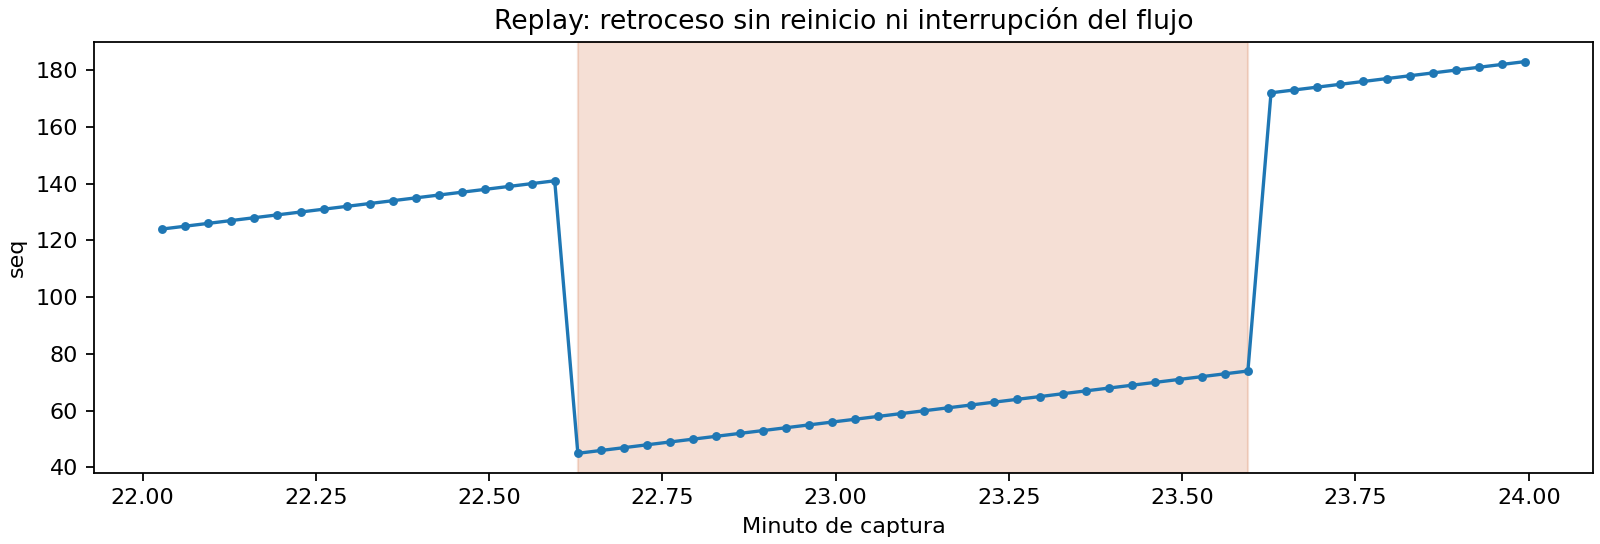
\includegraphics{figuras/replay.png}
\caption{Secuencia durante el replay}
\end{figure}

\hypertarget{b.-replay-frente-a-reconexiuxf3n}{%
\subsection{9b. Replay frente a
reconexión}\label{b.-replay-frente-a-reconexiuxf3n}}

\Needspace{4.5cm}
\begin{longtable}[]{@{}
  >{\raggedright\arraybackslash}p{(\columnwidth - 4\tabcolsep) * \real{0.3333}}
  >{\raggedright\arraybackslash}p{(\columnwidth - 4\tabcolsep) * \real{0.3333}}
  >{\raggedright\arraybackslash}p{(\columnwidth - 4\tabcolsep) * \real{0.3333}}@{}}
\toprule\noalign{}
\begin{minipage}[b]{\linewidth}\raggedright
Señal
\end{minipage} & \begin{minipage}[b]{\linewidth}\raggedright
Replay observado
\end{minipage} & \begin{minipage}[b]{\linewidth}\raggedright
Reconexión observada
\end{minipage} \\
\midrule\noalign{}
\endhead
\bottomrule\noalign{}
\endlastfoot
seq & Retrocede 141 a 45; luego 74 a 172 & Reinicia en 1 \\
t\_ms & Retrocede 282000 a 90000; luego 148000 a 344002 & Reinicia cerca
de 2000 \\
Intervalo ts & Mantiene recepción cercana a 2 s & Huecos de
15,724-24,830 s \\
Basura & No aparece alrededor del bloque & Una línea antes de cada
reconexión \\
Variables & 30 filas idénticas a un bloque anterior & Mediciones nuevas;
contadores reiniciados; coincidencias aisladas \\
\end{longtable}

\hypertarget{c.-disponibilidad-corregida}{%
\subsection{9c. Disponibilidad
corregida}\label{c.-disponibilidad-corregida}}

D\_corregida = 100 × (850 - 30) / 873 = \textbf{93,9290 \%}, manteniendo
Nesp como exige el enunciado. Disminuye 3,4364 puntos porcentuales
respecto de D inicial.

El Nperd inicial de 10 no reveló las tramas legítimas suprimidas porque
las 30 copias las sustituyeron una por una y se contaron en Nval. La
recepción continúa a 2 s y el máximo de seq de la sesión sigue siendo
213. El bloque reemplaza las seq legítimas 142-171, según los vecinos
141 y 172. Al descontar las copias quedan 40 tramas legítimas no
recibidas (10 pérdidas originales y 30 suprimidas), aunque la pregunta 4
contabilizaba únicamente 10.

\hypertarget{mitigaciuxf3n-y-costo-de-comunicaciuxf3n}{%
\section{10. Mitigación y costo de
comunicación}\label{mitigaciuxf3n-y-costo-de-comunicaciuxf3n}}

Se propone conservar CS para errores accidentales y agregar un contador
persistente de 64 bits, representado en 16 dígitos hexadecimales, y un
HMAC-SHA256 truncado a sus primeros 8 bytes (16 dígitos hexadecimales):

\begin{lstlisting}
$CPS,seq,t_ms,t_mcu,a0,pulsos,boton,ctr,mac*CS\r\n
\end{lstlisting}

ctr y mac son nombres de campos, no literales enviados. ctr tiene
siempre 16 caracteres; mac tiene siempre 16. Cada uno agrega una coma:
incremento total \textbf{34 bytes ASCII}. CS se recalcula sobre todo el
cuerpo, incluido mac, sin los delimitadores \$ y *.

El MAC se calcula con una clave compartida secreta sobre los bytes
exactos de CPS,\allowbreak seq,\allowbreak t\_ms,\allowbreak t\_mcu,\allowbreak a0,\allowbreak pulsos,\allowbreak boton,\allowbreak ctr (sin \$, sin coma
final ni mac). La representación debe ser canónica. El HMAC impide
aceptar modificaciones FDI sin la clave; el contador autenticado aporta
frescura y bloquea la repetición de mensajes ya aceptados. HMAC sin
contador no basta contra replay.

El receptor verifica estructura, CS y HMAC, y solo acepta ctr
estrictamente mayor al último contador aceptado de ese dispositivo. El
MAC se debe comparar en tiempo constante. Actualiza de manera atómica y
persistente el contador máximo junto con la aceptación del dato. Permite
saltos por pérdidas, pero rechaza valores iguales o inferiores. No debe
actualizar el máximo a partir de un mensaje sin autenticar. La clave y
el máximo deben sobrevivir a reinicios del receptor.

El Arduino debe garantizar que ctr no se reutilice tras un reinicio:
puede reservar bloques de contadores en memoria no volátil, con
actualización resistente a cortes de alimentación, para reducir
desgaste. Antes del desbordamiento se debe renovar la configuración de
forma autenticada. El HMAC no evita desconectar el cable ni que un nodo
comprometido con acceso a la clave emita mediciones falsas; requiere
proteger la clave.

\Needspace{4.5cm}
\begin{longtable}[]{@{}lrr@{}}
\toprule\noalign{}
Magnitud & Formato original & Formato autenticado \\
\midrule\noalign{}
\endhead
\bottomrule\noalign{}
\endlastfoot
L medio, con CRLF {[}bytes{]} & 32,625882 & 66,625882 \\
X {[}tramas/s{]} & 0,472781 & 0,472781 \\
R {[}bit/s{]} & 154,249023 & 314,994616 \\
Ocupación de 115200 baudios {[}\%{]} & 0,133897 & 0,273433 \\
\end{longtable}

Se usa L\_nuevo = L + 34 y la misma X de P5. La ocupación permanece por
debajo de 0,3 \%, aunque deben verificarse por separado memoria y tiempo
de cálculo del HMAC en el ATmega328P.

\hypertarget{cronologuxeda-cobertura-y-conclusiuxf3n}{%
\section{11. Cronología, cobertura y
conclusión}\label{cronologuxeda-cobertura-y-conclusiuxf3n}}

Los minutos se cuentan desde las 15:00:00. Los tiempos de la tabla se
obtuvieron de las muestras disponibles. Las pérdidas y los rechazos se
agrupan por tipo: sus intervalos abarcan la primera y la última
aparición, aunque no ocurren de manera continua.

\Needspace{14cm}
\begin{longtable}[]{@{}
  >{\raggedright\arraybackslash}p{(\columnwidth - 6\tabcolsep) * \real{0.2500}}
  >{\raggedright\arraybackslash}p{(\columnwidth - 6\tabcolsep) * \real{0.2500}}
  >{\raggedright\arraybackslash}p{(\columnwidth - 6\tabcolsep) * \real{0.2500}}
  >{\raggedright\arraybackslash}p{(\columnwidth - 6\tabcolsep) * \real{0.2500}}@{}}
\toprule\noalign{}
\begin{minipage}[b]{\linewidth}\raggedright
Evento
\end{minipage} & \begin{minipage}[b]{\linewidth}\raggedright
Inicio-fin {[}min{]}
\end{minipage} & \begin{minipage}[b]{\linewidth}\raggedright
Evidencia
\end{minipage} & \begin{minipage}[b]{\linewidth}\raggedright
Cobertura de detección
\end{minipage} \\
\midrule\noalign{}
\endhead
\bottomrule\noalign{}
\endlastfoot
Pérdidas sin recepción (10) & 1,027-29,758 & 7 aisladas y bloque de 3;
saltos sin rechazo & No CS; análisis seq/ts \\
Giro del potenciómetro & 4,027 & A0 pasa de \textasciitilde512 a
\textasciitilde1020 & No CS; análisis de A0 y registro del operador \\
Rechazos checksum (9) & 5,628-29,725 & XOR distinto; textos guardados &
Sí, checksum \\
Toques en D3 & 6,028-6,328 & boton sube de 0 a 31 & No CS; análisis del
contador y registro del operador \\
Giro del potenciómetro & 8,028 & A0 baja a \textasciitilde498 & No CS;
análisis de A0 y registro del operador \\
Rechazos truncada (4) & 8,528-19,261 & Mensajes incompletos & Estructura
del pipeline, antes del XOR \\
Desconexión USB 1 & 10,995-11,312 & Hueco 19,002 s; reinicio y basura &
No CS; correlación ts/seq/t\_ms/rechazos \\
Basura de arranque (3) & 11,253-25,198 & Texto sin \$ en tres
reaperturas & Primera condición del pipeline \\
FDI & 14,213-15,780 & 48 temperaturas elevadas incompatibles con ADC &
No CS; prueba ADC y tasa parcial \\
Desconexión USB 2 & 17,513-17,927 & Hueco 24,830 s; reinicio y basura &
No CS; correlación temporal \\
A0 flotante & 20,027-20,994 & Oscilaciones; detector hasta 21,028 & No
CS; detector físico con error de borde \\
Replay & 22,628-23,595 & 30 copias; retroceso sin hueco & No CS; JOIN y
continuidad \\
Desconexión USB 3 & 24,995-25,257 & Hueco 15,724 s; reinicio y basura &
No CS; correlación temporal \\
Toques en D3 & 27,024-27,324 & boton sube de 0 a 24 & No CS; análisis
del contador y registro del operador \\
\end{longtable}

En la implementación original, validar() por sí sola no identifica como
incidentes la entrada flotante, la FDI ni el replay. Las verificaciones
físicas y temporales de este informe son una capa adicional de análisis,
no capacidades del checksum. pulsos permanece en cero en todas las
tramas válidas; las alteraciones observadas de ese campo están en
mensajes rechazados.

Para los ataques encontrados, el punto más débil es el \textbf{canal sin
autenticación}, porque permite sustituir datos manteniendo un checksum
correcto. La mejora prioritaria es implementar HMAC más contador
persistente y su verificación en el nodo de borde. Debe complementarse
con alarmas de coherencia física para A0 y temperatura, y supervisión
temporal para las desconexiones. La disponibilidad sintáctica inicial de
97,3654 \% sobreestima la frescura de los datos: al eliminar replay baja
a 93,9290 \%, y todavía incluye las 48 tramas FDI y las mediciones
físicamente defectuosas.

\hypertarget{fuentes-y-reproducibilidad}{%
\section{Fuentes y reproducibilidad}\label{fuentes-y-reproducibilidad}}

Fuente de requisitos: Laboratorio Evaluado N.º 3, Análisis y Diseño de
Sistemas Ciber-Físicos, Universidad de Concepción, semestre 2026-2.
Fuentes de datos: captura\_nodo.txt y cps\_lab3\_respaldo.db
proporcionados para la actividad. Todas las cifras se calcularon sobre
esos archivos; no se incorporaron datos simulados.

Los scripts pipeline.py, analisis\_enlace.py y analisis\_fallas.py
reproducen la base, los gráficos y los CSV/JSON de resultados.
consultas.sql contiene las consultas utilizadas. Los criterios y
limitaciones de detección se documentan en P7-P9.

\hypertarget{anexo.-consultas-sql}{%
\section{Anexo. Consultas SQL}\label{anexo.-consultas-sql}}

\begin{lstlisting}[language=SQL]
-- P2: cantidad de filas de cada tabla.
SELECT COUNT(*) AS n_tramas FROM tramas;
SELECT COUNT(*) AS n_rechazos FROM rechazos;
SELECT causa, COUNT(*) AS cantidad FROM rechazos GROUP BY causa;

-- P3: ejecutar ATTACH una sola vez en la conexión.
ATTACH DATABASE 'cps_lab3_respaldo.db' AS ref;
SELECT COUNT(*) AS cantidad, SUM(seq) AS suma_seq, SUM(a0) AS suma_a0 FROM main.tramas;
SELECT COUNT(*) AS cantidad, SUM(seq) AS suma_seq, SUM(a0) AS suma_a0 FROM ref.tramas;
SELECT causa, COUNT(*) AS cantidad FROM main.rechazos GROUP BY causa;
SELECT causa, COUNT(*) AS cantidad FROM ref.rechazos GROUP BY causa;

-- Generada menos respaldo.
SELECT ts,seq,t_ms,t_mcu,a0,pulsos,boton FROM main.tramas
EXCEPT
SELECT ts,seq,t_ms,t_mcu,a0,pulsos,boton FROM ref.tramas;

-- Respaldo menos generada.
SELECT ts,seq,t_ms,t_mcu,a0,pulsos,boton FROM ref.tramas
EXCEPT
SELECT ts,seq,t_ms,t_mcu,a0,pulsos,boton FROM main.tramas;

-- P4: numeración por reinicios confirmados, no por cualquier caída de seq.
WITH numeradas AS (
  SELECT *, SUM(CASE WHEN seq=1 THEN 1 ELSE 0 END)
    OVER (ORDER BY id ROWS BETWEEN UNBOUNDED PRECEDING AND CURRENT ROW) AS sesion
  FROM tramas
)
SELECT sesion,COUNT(*) AS n_validas,MAX(seq) AS max_seq,MIN(ts) AS primera_ts,MAX(ts) AS ultima_ts
FROM numeradas GROUP BY sesion ORDER BY sesion;

WITH numeradas AS (
  SELECT seq,SUM(CASE WHEN seq=1 THEN 1 ELSE 0 END) OVER(ORDER BY id) AS sesion FROM tramas
), maximos AS (
  SELECT sesion,MAX(seq) AS max_seq FROM numeradas GROUP BY sesion
), conteos AS (
  SELECT (SELECT SUM(max_seq) FROM maximos) AS Nesp,
         (SELECT COUNT(*) FROM tramas) AS Nval,
         (SELECT COUNT(*) FROM rechazos WHERE causa IN ('checksum','truncada')) AS Ncorr
)
SELECT Nesp,Nval,Ncorr,Nesp-Nval-Ncorr AS Nperd,100.0*Nval/Nesp AS D_porcentaje FROM conteos;

-- P5: intervalos consecutivos calculados a partir de ts.
-- Se redondea al milisegundo para compensar el error de julianday.
WITH intervalos AS (
 SELECT ROUND((julianday(ts)-julianday(LAG(ts) OVER(ORDER BY id)))*86400,3) AS dt
 FROM tramas
)
SELECT SUM(dt<3) AS menor_3,
       SUM(dt>=3 AND dt<5) AS entre_3_y_5,
       SUM(dt>=5 AND dt<=10) AS entre_5_y_10,
       SUM(dt>10) AS mayor_10
FROM intervalos WHERE dt IS NOT NULL;



-- P6-P8: series y rechazos usados por el análisis Python.
SELECT * FROM tramas ORDER BY id;
SELECT * FROM rechazos ORDER BY id;
-- P9: igualdad del contenido con mensajes anteriores.
SELECT a.id,a.ts,a.seq,b.id AS id_original,b.ts AS ts_original
FROM tramas a JOIN tramas b
ON a.seq=b.seq AND a.t_ms=b.t_ms AND a.t_mcu=b.t_mcu
AND a.a0=b.a0 AND a.pulsos=b.pulsos AND a.boton=b.boton
AND b.id<a.id ORDER BY a.id;
\end{lstlisting}


\end{document}
